% grundlagen/grundlagen.tex
% Grundlagen zu raumpartitionierenden Datenstrukturen und Freiformflaechen
%
% Ausarbeitung zur Diplomarbeit Nr. 2035 - "Erzeugung und Evaluierung 
% von Oktalbaumstrukturen als Schnittstelle zu CAD-Programmen"
%
% Autor: Stefan Mahler 2002
%   Universitaet Stuttgart, SgS
% Betreuer: Ralf Mundani

\chapter{Darstellungsarten eines K"orpers}
\label{geombeschr}
%Basiswissen
%
%Octalbaeume, raumpartionierende Datenstrukturen, Vor-/Nachteile Octree
%(Datenstrukturen)
%
%Grundlagen der Freiformflaechen
%
%Bernstein, Spline, Casteljau (math. Grundlagen)

Die Beschreibung und Darstellung geometrischer K"orper wird als geometrische 
Modellierung bezeichnet. Zur rechnerorientierten Beschreibung solcher Modelle 
sind entsprechende Datenstrukturen erforderlich.

Im Weiteren wird ausschlie"slich die Modellierung von K"orpern mit
zeitlich fester Geometrie (also keine dynamischen Geometrien) behandelt.

Es gibt unterschiedliche Repr"asentationsm"oglichkeiten der geometrischen 
Verh"altnisse. Zur Bildung dreidimensionaler Modelle existieren 
kanten"~, fl"achen- und volumenorientierte Datenstrukturen. Diese besitzen 
verschiedene Eigenschaften.
Abschnitt \ref{modell_arten} gibt einen "Uberblick "uber wichtige 
Oberfl"achen- und Volumenmodelle und deren Eigenschaften.

Volumenmodelle werden auch als direkte Schemata bezeichnet. Die 
Information "uber die K"orpergeometrie und die Lokalisation der K"orper 
kann direkt aus dem Datenmodell extrahiert werden. Im Gegensatz dazu 
sind Oberfl"achen- und Kantenmodelle indirekte Schemata. Um die Gestalt 
eines K"orpers ermitteln zu k"onnen, m"ussen hier z.T. aufw"andige zus"atzliche 
Berechnungen erfolgen. Durch das Modell kann nicht sichergestellt werden,
dass die Datenstruktur nur Rigid-Bodies (die Randgebiete sind 
geschlossen; es gibt also z.B. beim Oberfl"achenmodell immer eine 
Begrenzungsfl"ache zwischen K"orperinnerem und -"au"serem) repr"asentiert.
Entsprechnend aufw"andig ist i.A. die Berechnung, ob sich ein Raumpunkt 
im K"orperinneren befindet oder nicht.
Je nach Fachgebiet werden bestimmte Repr"asentationsformen bevorzugt, die 
f"ur die jeweilige Anwendung am besten geeignet scheinen.
Kantenorientierte Darstellungen sind f"ur die Darstellung eindimensionaler 
Geometrieen gut geeignet. 
Volumen- und Oberfl"achenmodelle sind in der Lage, auch komplexe 
dreidimensionale Objekte zu beschreiben. W"ahrend bei der geometrischen 
Modellierung Oberfl"achenmodelle zumeist in CAD-Systemen verwendet werden, 
kommen bei Simulationen h"aufig Berechnungsgitter zum Einsatz, die durch 
r"aumliche Diskretisierung erzeugt wurden, also spezielle Volumenmodelle.
Die Nutzung unterschiedlicher geometrischer Modelle ist eines der gr"o"sten
Hindernisse zur Integration u.a. von CAD und Simulation.
Abschnitt \ref{schnittstelle_octree} erkl"art die Besonderheiten der 
Oktalbaumstruktur, die es erm"oglichen, sie als Schnittstelle zwischen 
CAD und Simulation zu verwenden.

% grundlagen/modell_arten.tex
% Wichtige Oberflaechen- und Volumenmodelle
%
% Ausarbeitung zur Diplomarbeit Nr. 2035 - "Erzeugung und Evaluierung 
% von Oktalbaumstrukturen als Schnittstelle zu CAD-Programmen"
%
% Autor: Stefan Mahler 2002
%   Universitaet Stuttgart, SgS
% Betreuer: Ralf Mundani

\section{Wichtige Oberfl�chen- und Volumenmodelle}
\label{modell_arten}
%Oberflaechen: Trianguliert, Freiformflaechen
%(Bernstein, Spline, Casteljau (math. Grundlagen))
%
%Volumen: CSG, Normzellenschema, raumpartionierende Datenstrukturen
Der folgende Abschnitt widmet sich den wichtigsten Oberfl"achen- und 
Volumenmodellen. Umfangreichere Beschreibungen liefern 
\cite{bungartz, comp_graf, aumann_spitzmueller, pareigis, abramowski}.

\subsection{Oberfl"achenmodelle}
\label{flmodels}
Von Oberfl"achendarstellungen spricht man, wenn ein Objekt nicht durch 
sein Volumen, sondern -- indirekt -- durch die das Objekt begrenzenden Fl"achen 
beschrieben wird. Sie werden deshalb auch boundary representations oder 
kurz B-Rep genannt. 

Allerdings repr"asentiert nicht jede Ansammlung von Fl"achen einen 
starren K"orper im Sinne der geometrischen Modellierung. Hiermit ist gemeint, 
dass f"ur jeden beliebigen Raumpunkt entschieden werden kann, ob er sich
innerhalb, au"serhalb oder auf der Oberfl"ache des K"orpers befindet. Um dies 
zu gew"ahrleisten, m"ussen weitere Bedingungen erf"ullt sein:
\begin{enumerate}
\item \label{oberflbed_geschl}\textbf{Geschlossenheit:}
    Jeder Kantenpunkt ist Randpunkt zweier Fl"achen. Eckpunkte werden 
    von jeweils mindestens drei Fl"achen gebildet. 
    Der Rand einer jeder Fl"ache besitzt 
    genauso viele Kanten wie Eckpunkte. Es gibt also insbesondere keine 
    Unterbrechungen in den Kanten oder L"ocher in den Fl"achen, es sei denn, 
    dass der Lochrand von weiteren Fl"achen, wie bei einem Hohlzylinder,
    ummandelt ist.
\item \label{oberflbed_orientiert}\textbf{Orientierheit der Oberfl"achen:}
    Eine Fl"ache ist dann orientierbar, wenn sie zwei wohlunterscheidbare 
    Seiten besitzt.
    Bedingung \ref{oberflbed_geschl} und Bedingung \ref{oberflbed_noselfcut}
    garantieren zusammen die Orientierbarkeit der Oberfl"achen.
\item \label{oberflbed_noselfcut}\textbf{Kein Eigenschnitt:}
    Es muss noch gew"ahrleistet sein, dass die Fl"achen und K"orper 
    sich nicht selbst 
schneiden.
\end{enumerate}
Sind alle drei Bedingungen erf"ullt, kann durch die Orientierung der Fl"achen 
festgelegt werden, welche Punkte sich innerhalb bzw. au"serhalb eines K"orpers
befinden. Besteht das Oberfl"achenmodell aus mehreren Zusammenhangskomponenten,
ist dies auch notwendig, um entscheiden zu k"onnen, ob es sich z.B. hierbei um 
ein Hohlk"orper oder mehrere K"orper handelt, da sonst eventuell mehrere 
Zuordnungsm"oglichkeiten von K"orper"au"serem und K"orperinnerem bestehen.

Als Teilfl"achen sind im einfachsten Fall Dreiecke m"oglich. Diese Form der 
Modellierung eines K"orpers wird auch als Triangulierung bezeichnet.
Die K"orperoberfl"achen werden also hierbei durch Dreiecksnetze approximiert.
Der Vorteil des Einsatzes von Dreiecksnetzen liegt in dem in Vergleich zu
anderen Oberfl"achenmodellen relativ einfachen Handling der Geometrie:
\begin{itemize}
\item Zur Beschreibung eines Dreiecks sind immer genau $3$ Eckpunkte 
    erforderlich, woraus sich eine einfache Struktur f"ur ein 
    Oberfl"achenelement 'Dreieck' ergibt.
\item Dreiecke spannen immer eine Ebene auf, die durch die $3$ Punkte genau
    beschrieben werden. (Bei Vierecken beispielsweise k"onnte der vierte 
    Eckpunkt au"serhalb der Ebene, die durch die $3$ anderen Eckpunkte 
    aufgespannt wird, liegen.)
\item Dreiecke sind stets konvexe Polygone. F"ur den Test, ob ein Punkt
    innerhalb oder au"serhalb eines Dreiecks liegt, gibt es aufgrund dieser 
    Eigenschaft effiziente Algorithmen.
\item Welche Seite des Dreiecks K"orperau"senfl"ache und welche Innenfl"ache 
    ist, l"asst sich leicht aus den drei Eckpunkten bestimmen, wenn folgende 
    Festlegung bez"uglich der Reihenfolge der Eckpunkte eingehalten wird: \\
    Der Normalenvektor der Ebene \(\vct{n_E}\), 
    der durch die Vektoren aufgespannt wird, die sich zwischen zweiten ($B$) 
    bzw. drittem Eckpunkt ($C$) als Endpunkte und dem ersten Eckpunkt ($A$) 
    als Anfangspunkt ergeben:
    \gl{gl_flaechenorientierung}{\vct{n_E} ~ = ~ {\vct{AB} \crossprod \vct{AC}
	 \over |\vct{AB}| ~ |\vct{AC}| }\mbox{,}}
    ist immer in Richtung des K"orper"au"seren gerichtet. 
\end{itemize}
Besitzt ein K"orper eine Oberfl"ache mit starken Kr"ummungen, so m"ussen die 
Dreiecke sehr klein gew"ahlt werden, um den K"orper "uberhaupt approximieren 
zu k"onnen. Das erzeugte Modell wirkt kantig, obwohl der zu modellierende 
K"orper (z.B. bei einer Kugel) keine Kanten besitzt. Meist werden jedoch 
stetige Verl"aufe und nicht kantige Modelle ben"otigt. 
Zur Beschreibung von K"orpern mit gekr"ummter Oberfl"ache werden daher h"aufig 
Freiformkurven-/fl"achen zur Modellierung eingesetzt. Die Nutzung von 
Freiformfl"achen erlaubt die exakte Modellierung von Kugeln, Kegeln und 
Kugel-/Kegelteil\-k"orpern. Freiformkurven-/fl"achen eigenen sich 
insbesondere f"ur die geometrische Modellierung der h"aufig ben"otigten
\contii-stetigen\footnote{Die Kurve/Fl"ache ist zwei Mal (partiell) 
differenzierbar. Die zweite Ableitung ist stetig.} Verl"aufe.

Im Folgenden wird auf die Freiformtypen \bez-Kurven, B-Splines
und NURBS eingegangen. Anschlie"send wird die Freiformfl"achenerzeugung aus 
dem Freiformkurven-Schema hergeleitet. F"ur weiterf"uhrende Erl"auterungen ist
\cite{farin} zu empfehlen. \cite{boor, boor2} geben n"ahere  
Erl"auterungen f"ur das Verst"andnis von Splinefunktionen. Hier werden 
Algorithmen zum Einf"ugen und L"oschen von Knoten ausf"uhrlich beschrieben. 
\cite{nurbs_book} gibt eine ausf"uhrliche und dennoch "ubersichtliche
Darstellung wesentlicher Zusammenh"ange zwischen \bez-Kurven/-Fl"achen, 
Splines und NURBS. Es werden f"ur den Umgang wichtige Algorithmen
vorgestellt. Das Buch enth"alt auch praktische Tipps zur Anwendung der 
Algorithmen und Implementierungen der Verfahren im C-Code.

Um neben glatten Oberfl"achen auch gekr"ummte Verl"aufe modellieren zu 
k"onnen, wird nun die lineare Darstellung zu einer polynomiellen erweitert. 
Polynome besitzen f"ur die Modellierung gekr"ummter Verl"aufe viele geeignete 
Eigenschaften:
\begin{itemize}
\item Sie sind "uber den ganzen Bereich der reellen Zahlen definiert und sind 
    $n$-mal differenzierbar, wenn $n$ der Grad des Polynoms ist. 
    Sie haben also insbesondere keine Unstetigkeitsstellen oder 'Knickstellen'.
\item Mit $n+1$ Punkten k"onnen beliebige Polynome $n$-ten Grades eindeutig 
    dargestellt werden und umgekehrt.
\item Polynome sind relativ leicht berechenbar. Es m"ussen also keine 
    aufw"andigen Berechnungsroutinen implementiert werden. Des Weiteren sind 
    Polynome einfach analysierbar.
\item Lineare Funktionen k"onnen als Polynome ersten Grades aufgefasst werden 
    und sind somit nur ein spezielles Polynom.
\end{itemize}
Die polynomielle Interpolation erweist sich jedoch in vielen F"allen als 
ung"unstig, da sie f"ur Polynome h"oheren Grades im Allgemeinen 
unerw"unschte numerische Eigenschaften besitzt:
Die Funktion ist schlecht konditioniert. Kleine lokale "Anderungen haben 
starke globale Ver"anderung. Diese Ver"anderungen sind nicht intuitiv. Schon 
deshalb ist dieser Ansatz f"ur den konstruktiven Entwurf unbrauchbar.

%\begin{samepage}
Daraus ergeben sich zwei Kriterien:
\begin{description}
\item[Kontrollierbarkeit:] Ver"anderungen der Kurven-/Fl"achen-Parameter
    f"uhren zu voraussagbaren und kontrollierbaren Effekten bez"uglich
    der Kurvengestalt.
\item[Lokalit"atsprinzip:]
    Lokale Ver"anderungen bedingen maximal nur geringe globale Ver"anderungen.
    Verschiebt man z.B. einen Kontrollpunkt, so ver"andert sich
    der Verlauf entfernter Kurven-/Fl"achenst"ucke nur wenig oder 
    --~idealerweise~-- garnicht.
\end{description}
Die drei Approximationsverfahren, die Modellierung durch \bez-Kurven, Splines
und NURBS, erf"ullen diese beiden Kriterien.
%\end{samepage}

%%%%%%%%%%%%%%%%%%%%%%%%%%%%%%%%%%

% grundlagen/bezier.tex
% Bezier-Kurven
%
% Ausarbeitung zur Diplomarbeit Nr. 2035 - "Erzeugung und Evaluierung 
% von Oktalbaumstrukturen als Schnittstelle zu CAD-Programmen"
%
% Autor: Stefan Mahler 2002
%   Universitaet Stuttgart, SgS
% Betreuer: Ralf Mundani

\subsubsection{\bez-Kurven}
\label{bezier}
%-Bernstein-Polynome
%-Casteljau-Algorithmus
%-Zusammengesetzte Bezier-Kurven

Eine Kurve, die durch 
\gl{gl_bezier_kurve}{{\bf x}(t) = \sum_{i=0}^n ~B_i^n(t)~{ \bf b}_i\mbox{, }~
    ~t \in{} [0, 1]}
beschrieben wird, wird als \bez-Kurve bezeichnet. Dabei sind die 
Bernstein-Polynome $ B_i^n $ definiert durch
\gl{gl_bernstein_2d}{B_i^n(t) = \binom{n}{i} ~(1 - t)^{n-i}~t^i\mbox{, }~ 
    ~t \in{} [0, 1]\mbox{, }~i= 0,\dots,n\mbox{.}}
Damit gilt
\gl{gl_sum_bernstein_eins}{\sum_{i=0}^n B_i^n(t) = 1\mbox{, }~
    ~\forall{} t \in [0, 1]}
und 
\gl{gl_bernstein_rand_a}{B_0^n(0) = B_n^n(1) = 1} bzw.
\gl{gl_bernstein_rand_b}{B_0^n(1) = B_n^n(0) = 0\mbox{.}}

\bez-Kurven sind die einfachste Form einer symmetrischen Darstellung 
durch polynomielle Approximation mit Kontrollpunkten. Die 
Kontrollpunkte ${\bf b}_i$ einer \bez-Kurve werden \bez-Punkte genannt. 
Sie bilden ein Kontrollpolygon.
\bez-Kurven besitzen folgende wichtige Eigenschaften: \label{bez_props}
\begin{enumerate}
\newcommand\nritem[2]{\item \textbf{#1:} \label{#2}}
\nritem{Konvexe-H"ullen-Eigenschaft}{bez_prop_convex_hull}
    Eine \bez-Kurve liegt in der konvexen H"ulle ihres Kontrollpolygons.
\nritem{Stetigkeit, Differenzierbarkeit}{bez_prop_diff}
    \bez-Kurven sind stetig. Besitzt die \bez-Kurve Mehrfachkontrollpunkte 
    oder besitzt der die Kontrollpunkte miteinander verbindende Kantenzug 
    Schleifen (das Kontrollpolygon ist also nicht konvex), kann die Kurve 
    jedoch an einigen Stellen eventuell nicht differenzierbar sein.
\nritem{Interpolation der Kurvenenden}{bez_prop_intpol_kurvend}
    Kontrollpolygon und \bez-Kurve stimmen in Anfangs- und Endpunkt 
    "uberein. Die inneren \bez-Punkte werden i.A. nur approximiert und 
    liegen somit dann auch nicht auf der \bez-Kurve.
\nritem{Kurvenanstieg an den Kurvenenden}{bez_prop_diff_kuvend}
    Die Strecken $\overline{{\bf b}_0{\bf b}_1}$ und 
    $\overline{{\bf b}_{n-1}{\bf b}_n}$ des Kontrollpolygons verlaufen im 
    Anfangs- und Endpunkt tangential zur \bez-Kurve.
\nritem{Einfluss von Kontrollpunkten, Globale Modifikation}{bez_prop_cp_einfl}
    ${\bf b}_i$ hat den gr"o"sten Einflu"s auf ${\bf x}(t)$ bei $t = i/n$. 
    Bis auf Anfangs- und Endpunkt der Bezierkurve werden zur Berechung 
    eines Kurvenpunkts \emph{alle} Kontrollpunkte (wenn auch in 
    unterschiedlichem Ausma"s) ber"ucksichtigt.
    Die Modifikation eines Kontrollpunktes wirkt sich global auf die
    \bez-Kurve aus.
\nritem{Formerhaltungs-Eigenschaft}{bez_prop_formerh}
    Ist das Kontrollpolygon konvex, so ist es auch die \bez-Kurve.
\nritem{Beschr"ankte Schwankung}{bez_prop_beschr_schw}(auch \emph{variation
    diminishing} genannt)
    Keine Gerade schneidet die \bez-Kurve "ofter als das entsprechende 
    Kontrollpolygon.
    Daraus ist auch direkt die Eigenschaft der \emph{linearen Pr"azision} 
    ableitbar: Liegen die Kontrollpunkte ${ \bf b}_0, \dots, { \bf b}_n$ einer 
    \bez-Kurve kollinear, dann liegt die \bez-Kurve auf der Strecke 
    $\overline{{\bf b}_0{\bf b}_n}$.
\nritem{Graderh"ohung}{bez_prop_grad_incr}
    Bei fortgesetzter Graderh"ohung durch Einf"ugen zus"atzlicher 
    Kontrollpunkte konvergiert das Kontrollpolygon gegen die \bez-Kurve.
\nritem{Affine Invarianz}{bez_prop_aff_inv}
    \bez-Kurven sind bez"uglich Rotation, Skalierung ($\not= 0$), Spiegelung 
    und Translation invariant.
\end{enumerate}

Eine effiziente und numerisch stabile M"oglichkeit zur Berechnung der 
Kurvenpunkte ${ \bf x}(t)$ ist der \emph{Algorithmus von de Casteljau}. 
Abbildung \ref{abb_alg_casteljau} zeigt ein Schema zur geometrischen 
Konstruktion von ${\bf x}(t=\frac{2}{3})$ f"ur $n=3$ nach diesem Algorithmus. 

\graf{abb_alg_casteljau}{Algorithmus von de Casteljau (\emph{geom.})}{%
    casteljau}

Die Eigenschaften \ref{bez_prop_diff} und \ref{bez_prop_cp_einfl} k"onnen sich 
nachteilig auf die Modellierung von \bez-Kurven auswirken. Diese Nachteile 
wie mangelnde Diffenrenzierbarkeit und unerw"unschte Ausgleichseffekte von 
Kontrollpunkten infolge fehlender Lokalit"at der Kontrollpunktwirkung werden 
h"aufig bei h"ohergradigen \bez-Kurven sichtbar. Zudem sind mathematische 
Beschreibungen der \bez-Kurven vom Grad $\ge 10$ unhandlich, Berechnungen sind 
rechenzeitintensiv. Andereseits erfordert das Nachbilden komplexer realer 
Kurven evtl. viele Kontrollpunkte. 

Einen Ausweg bieten \textbf{zusammengesetzte \bez-Kurven}. Die Gesamtkurve 
wird aus einzelnen Kurvensegmenten gleichen Grads zusammengesetzt. 
Das Segment $i$ der \bez-Kurve besteht somit aus den Kontrollpunkten 
${\bf b}_{0,i}, \dots, {\bf b}_{p, i}$, wenn die Segmente vom Grad $p$ sind. 
Nun wird zweckm"a"siger Weise ein Verfahren ben"otigt, was zu einem globalen 
Parameter $u$ eindeutig den lokalen Parameter $t$ des $i$-ten Segments 
bestimmt. O.B.d.A. sei angenommen, dass die Gesamtkurve normalisiert, also 
$u \in [0, 1]$, sei. L"auft $u$ somit "uber $[0, 1]$ wird die Gesamtkurve 
"uberstrichen. Mit Hilfe der Zerlegung $0=u_0<u_1<\dots<u_n<u_{n+1}=1$ des 
Intervalls $[0, 1]$ kann das $i$-te Segment "uber dem Intervall 
$I_i = [u_i, u_{i+1}]$ definiert werden. Der lokale Paramterwert $t$ des 
Intervalls $I_i$ kann dann mit
\gl{gl_def_t_durch_u}{t = {{u - u_i} \over {u_{i+1} - u_i}}\mbox{, }~
    ~u \in{} [u_i, u_{i+1}]}
definiert werden. 

Wegen Eigenschaft \ref{bez_prop_intpol_kurvend} l"asst 
sich die Stetigkeit von zusammengesetzten \bez-Kurven leicht bewerkstelligen: 
Hierf"ur m"ussen die Anfangspunkte des nachfolgenden Segments nur mit den 
jeweiligen Endunkten des Vorg"angersegments "ubereinstimmen:
\gl{gl_bez_zusammenges_cnt}{{ \bf b}_{n, i} = { \bf b}_{0, i+1}\mbox{.}} 
Schwieriger l"asst sich allerdings hinreichende Differenzierbarkeit an den 
Segment"uberg"angen gew"ahrleisten. Um an den Segment"uberg"angen 
\conti-Stetigkeit zu erhalten, muss
\gl{gl_bez_picewise_diff}{
    {{{ \bf b}_{n, i} - { \bf b}_{n-1, i}} \over {u_{i+1} - u_i}} 
    = {{{ \bf b}_{1, i+1} - { \bf b}_{n, i}} \over {u_{i+2} - u_{i+1}}}}
gelten. Dies bedeutet, dass die drei Punkte ${\bf b}_{n-1, i}$, 
${\bf b}_{n, i}={\bf b}_{0, i+1}$ und ${\bf b}_{1, i+1}$ kollinear sein 
m"ussen \emph{und} dass ${\bf b}_{n, i}$ die Strecke 
$\overline{{\bf b}_{n-1, i}{\bf b}_{1, i+1}}$ im Verh"altnis 
\hbox{\((u_{i+1} - u_i) : (u_{i+2} - u_{i+1})\)} teilt. 
Um die h"aufig geforderte \contii-Stetigkeit zu erhalten, muss das Schema 
unter Einbeziehung der Punkte ${\bf b}_{n-2, i}$ und ${\bf b}_{2, i+1}$ 
entsprechend erweitert werden. 

Nachteilig an zusammengesetzten \bez-Kurven ist, dass die ersten und letzten 
Kontrollpunkte eines jeden Segments die Bedingungen 
\glref{gl_bez_zusammenges_cnt} und \glref{gl_bez_picewise_diff} erf"ullen 
m"ussen, um die Differenzierbarkeit der Gesamtkurve sicherzustellen. Daf"ur 
m"ussen eventuell zus"atzliche Kontrollpunkte eingef"ugt werden. Dieses 
Problem kann durch die Nutzung von B-Spline-Kurven umgangen werden.

%% End of Document


% grundlagen/splines.tex
% B-Splines
%
% Ausarbeitung zur Diplomarbeit Nr. 2035 - "Erzeugung und Evaluierung 
% von Oktalbaumstrukturen als Schnittstelle zu CAD-Programmen"
%
% Autor: Stefan Mahler 2002
%   Universitaet Stuttgart, SgS
% Betreuer: Ralf Mundani

\subsubsection{B-Splines}
\label{spline}
%-De-Boor-Algorithmus
%-B-Spline-Funktionen
%-B-Spline-Kurven
B-Spline-Kurven vom Grad $p$ sind definiert durch
\gl{gl_b_spline_kurve}{{\bf x}(u) = \sum_{i=0}^{n}~ N_i^p(u)~
    { \bf c}_i\mbox{,}}
wobei ${ \bf c}_i$ die Kontrollpunkte und $N_i^p$ die zur B-Spline-Kurve 
geh"origen Basisfunktionen "uber den Knotenvektor $U = \{u_0, \dots, u_n\}$ 
darstellen. Analog zu den zusammengesetzten \bez-Kurven ist $u_{\min} = u_0 < 
u_1 < \dots < u_n = u_{\max}$ eine Zerlegung des Intervalls $[u_{\min}, 
u_{\max}]$. 
Wieder ergeben sich Teilkurven zu jedem Teilintervall. Die Glattheit der 
Gesamtkurve ist hier jedoch auch "uber die Sto"sstellen der Teilkurven 
gesichert, da B-Spline-Basisfunktionen anstelle der Bernsteinpolynome 
verwendet werden. 

Die Basisfunktionen $p$-ter Ordnung $N_i^p$ k"onnen ausgehend von der 
Basisfunktion erster Ordnung $N_i^1$
\gl{gl_basis_fkt_lin}{%
    N_i^1(u) = \left\{
    \begin{array}{rl}
	1 & u_i \le u < u_{i+1}\\
	0 & \mbox{sonst}~
    \end{array} \right.
    ~(0 \le i < n)}
rekursiv mit
\gl{gl_basis_fkt_rek}{N_i^p(u) = {{u - u_i}\over{u_{i+p-1} - u_i}}~N_i^{p-1}(u) 
    + {{u_{i+p} - u}\over{u_{i+p} - u_{i+1}}}}
berechnet werden. 
Alle Terme $(u_i-u)/(u_{i+p-1}-u_i)$ und $(u_{i+p}-u)/(u_{i+p}-u_{i+1})$ 
werden f"ur $u_{i+p-1}=u_i$ bzw. $u_{i+p}=u_{i+1}$ mit $0$ festgelegt.
Somit gilt 
\gl{gl_sum_basisfuns_eins}{\sum_{i=0}^{n-p} N_i^p(u) = 1\mbox{,}~
    ~\forall{} u \in [u_{p-1}, u_{n-p+1}]}
und
\gl{gl_basis_funs_null_gr_null}{N_i^p(u) \left\{
    \begin{array}{rl}
	> 0 & u \in (u_i, u_{i+p})\\
	= 0 & \mbox{sonst.}
    \end{array} \right.}

Mit Hilfe des \emph{de-Boor-Algorithmus} k"onnen B-Spline-Kurven beliebigen 
Grades ohne Kenntnis der Basisfunktionen erzeugt werden. Er ist das 
"Aquivalent des Algorithmus von Casteljau f"ur B-Spline-Kurven:
Sei eine B-Spline-Kurve $p$-ten Grades durch die Kontrollpunkte 
${\bf c}_0, \dots, {\bf c}_n$ mit zugeordneten Parameterwerten 
$u_0, \dots, u_n$, wobei $u_{\min} = u_0 < \dots < u_n = u_{\max}$ ist, 
gegeben. 

Setzt man 
${\bf b}_i^{(0)} = \cases{ {\bf c}_i & i \in [0, n]\\
			   0	     & \mbox{sonst,} }$
dann enth"alt ${\bf b}_{\phi}^{(p-1)}(u)$ nach $p-1$-maliger Anwendung der 
Rekursionsformel
\gl{gl_de_boor}{{\bf b}_i^{(r)}(u) = {{u_{i+p-r} - u}\over{u_{i+p-r} - u_i}}~
    { \bf b}_{i-1}^{(r-1)}(u) + {{u - u_i}\over{u_{i+p-r} - u_i}}~
    { \bf b}_{i}^{(r-1)}(u)}
den Punkt der B-Spline-Kurve zu $u$ mit $u \in [u_{\phi}, u_{\phi+1}]$ und 
$0 \le \phi < n$.
Substituiert man 
\gl{gl_subst_u_term}{\alpha_i^r = {{u - u_i}\over{u_{i+p-r} - u_i}}}
erh"alt man die zum Algorithmus von Casteljau analoge Darstellung
\gl{gl_de_boor_Subst}{{ \bf b}_i^{(r)} = (1 - \alpha_i^r)~
    { \bf b}_{i-1}^{(r-1)} + \alpha_i^r~{ \bf b}_i^{(r-1)}\mbox{.}}
Mit $p = n + 1$, dem Knotenvektor $U = \{0, \underbrace{1, \dots, 1}_{n}\}$ 
und $u_{-n} = \dots = u_{-1} = u_{\min}$ ergibt sich $\alpha_i^r = u$.
\bez-Kurven sind somit nur ein Spezialfall von B-Spline-Kurven.

B-Splines besitzten viele Eigenschaften von \bez-Kurven 
(vgl. Seite \pageref{bez_props}):
\begin{itemize}
\item Konvexe-H"ullen-Eigenschaft (sogar in strengerer Form)
\item Invarianz bez"uglich affiner Transformationen 
\item Endpunkt-Interpolation, falls die ersten bzw. letzten $p+1$ Knoten den 
    gleichen Wert besitzen
\item Kontrollpunkt-Symmetrie
\item Formerhaltungs-Eigenschaft 
\item Beschr"ankte Schwankung (variation diminishing)
\end{itemize}

Hinzu kommt die lokale Tr"agereigenschaft 
(vgl. \glref{gl_basis_funs_null_gr_null}): 
Modifikationen an einem Kontrollpunkt bleiben auf $p$ Nachbarn (bei einer 
B-Spline-Kurve $p$-ten Grades) begrenzt.

Allerdings sind B-Splines wie \bez-Kurven \emph{nicht} invariant bez"uglich 
projektiven Abbildungen. Diesen Nachteil kann man durch NURBS beseitigen.

%% End of Document


% grundlagen/nurbs.tex
% NURBS
%
% Ausarbeitung zur Diplomarbeit Nr. 2035 - "Erzeugung und Evaluierung 
% von Oktalbaumstrukturen als Schnittstelle zu CAD-Programmen"
%
% Autor: Stefan Mahler 2002
%   Universitaet Stuttgart, SgS
% Betreuer: Ralf Mundani

\subsubsection{NURBS}
\label{nurbs}
%- projektive Invarianz
%- Einf"uhren von Gewichten
NURBS ist die Kurzform f"ur \emph{Non Uniform Rational B-Splines}. 
Wie schon aus den Namen hervorgeht, werden hier im Gegensatz zu \bez-Kurven 
und Splines rationale Funktionen zur Beschreibung verwendet. 
NURBS sind definiert durch
\gl{gl_nurbs}{{ \bf x}(u) = {\scriptstyle{\sum^n_{i=0}} ~ N_i^p(u) ~ w_i 
    ~ { \bf c}_i \over \scriptstyle{\sum^n_{i=0}} ~ N_i^p(u) ~ w_i}\mbox{.}}
Den Kontrollpunkten ${\bf c}_i$ werden noch zus"atzlich Gewichte $w_i$ 
zugeordnet, die "uberlicherweise als Formparameter verwendet werden.
Je gr"o"ser das Gewicht eines Kontrollpunkts ist, desto st"arker ist sein 
Einfluss auf den Kurvenverlauf, indem sich die NURBS-Kurve st"arker diesem 
Kontrollpunkt ann"ahert.

Werden allerdings alle Gewichte um den gleichen Faktor ver"andert, "andert das 
nichts am Verlauf der NURBS-Kurve. Besitzen alle Kontrollpunkte das gleiche 
Gewicht, so ergibt das wieder die 'gew"ohnliche' B-Spline. B-Splines (und 
somit auch \bez-Kurven) sind also Spezialf"alle von NURBS.

Eine NURBS-Kurve kann man sich als eine in den 3-dimesionalen Raum projezierte 
4-dimensionale B-Spline-Kurve vorstellen.
Wie sich zeigen l"asst, sind NURBS-Kurven bez"uglich projektiven Abbildungen 
invariant.

\bez-Kurven, B-Splines und NURBS besitzen somit i.A. unterschiedliche 
Eigenschaften. Andererseits sind ihre Datenstrukturen unterschiedlich komplex. 
Es existieren Algorithmen zum Konvertieren geometrischer Modelle von 
NURBS-Darstellung in \bez-Kurven. Die drei Darstellungsformen \bez-Kurven, 
B-Splines und NURBS sind somit gleichm"achtig. Je nach Aufgabenstellung 
kann es evtl. g"unstig sein, vor der Bearbeitung des Modells die eine in eine 
andere Darstellungsform umzuwandeln.

%% End of Document


% grundlagen/k2flaechen.tex
% kurven ==> Fleachen
%
% Ausarbeitung zur Diplomarbeit Nr. 2035 - "Erzeugung und Evaluierung 
% von Oktalbaumstrukturen als Schnittstelle zu CAD-Programmen"
%
% Autor: Stefan Mahler 2002
%   Universitaet Stuttgart, SgS
% Betreuer: Ralf Mundani

\subsubsection{Fl"achenerzeugung aus Kurven}
\label{freiform}
Im folgenden Abschnitt soll es um die Gewinnung von Fl"achen aus Kurven gehen. 
Analog zum \emph{Verschiebegeometrieschema} \vpageref{vschiebgeom}, wo aus 
einem 2D-Objekt, welches entlang einer Kurve verschoben wird, ein 3D-Objekt 
erzeugt wird, k"onnte hier aus einer Kurve (1D) eine Fl"ache (2D) erzeugt 
werden. 

\paragraph{Coons Patch}~\\
Im einfachsten Fall lassen sich 
Vierecke $P_1P_2P_4P_3$ durch Verschieben 
der Strecke $\overline{P_1P_2}$ auf geradem Weg nach $\overline{P_3P_4}$ 
generieren. Ein Viereckspunkt $x_{s,t}$ wird dann durch die Gleichung
\gl{gl_viereckspunkt}{{\bf x}_{s,t}(s, t) = (1 - s) (1 - t) {~\bf P}_1 
    + s (1 - t) {~\bf P}_2 + (1 - s) t {~\bf P}_3 + s t {~\bf P}_4}
beschrieben, wobei $s, t \in [0, 1]$ sind. Es stellt den linearen Fall
des Tensorprodukts dar. Allgemein l"asst sich die Gleichung
\gl{gl_allg_fl}{{\bf x}(s, t) = { \bf x}_s(s, t) + { \bf x}_t(s, t)
    - { \bf x}_{s,t}(s, t)}
ermitteln. Hierbei ist
\gl{gl_fl_kv_xs}{{\bf x}_s(s, t) = g_0(t) { \bf \gamma}_0(s)
    + g_1(t) { \bf \gamma}_1(s)}
und
\gl{gl_fl_kv_xt}{{\bf x}_t(s, t) = f_0(s) { \bf \delta}_0(t) 
    + f_1(s) { \bf \delta}_1(t)\mbox{,}} 
wobei $f_0(s) + f_1(s) = 1$ ($s \in{} [0, 1]$) und 
$f_0(0) = f_1(1) = 1$ bzw. $g_0(t) + g_1(t) = 1$ ($t \in{} [0, 1]$) 
und $g_0(0) = g_1(1) = 1$ ist. ${\bf \gamma}_0$, ${\bf \gamma}_1$, 
${\bf \delta}_0$ und ${\bf \delta}_1$ bilden die Randkurven, 
$f_0$, $f_1$, $g_0$ und $g_1$ sind allgemeine Interpolationskurven.
Der Anteil ${\bf x}_{st}$ ist sowohl in ${\bf x}_s$ als auch in 
${\bf x}_t$ enthalten und muss deshalb von der Summe wieder abgezogen 
werden, um nicht f"alschlicher Weise doppelt aufgerechnet zu werden.

\paragraph{\bez-Fl"achen}~\\
Unter Nutzung von Bernstein-Polymen ${\bf b}_{i,k}$ ergibt sich mit 
\glref{gl_bezier_kurve}
\gl{gl_bezier_fl}{{\bf x}(s, t) = \sum_{i=0}^{n} \sum_{k=0}^{m}~ 
    B_i^{n}(s)~B_k^{m}(t)~{ \bf b}_{i,k}\mbox{, }~	
	~s, t \in{} [0, 1]\mbox{,}} 
wobei die \bez-Punkte ${\bf b}_{i,k}$ das zur \bez-Fl"ache zugeh"orige 
Kontrollnetz aufspannen.

\paragraph{B-Spline-Fl"achen}~\\
Analog ergibt sich f"ur B-Spline-Fl"achen mit \glref{gl_b_spline_kurve}
\gl{gl_spline_fl}{{\bf x}(s, t) = \sum_{i=0}^{n}\sum_{k=0}^{m}~ 
    N_i^p(s)~N_k^q(t)~{ \bf c}_{i,j}\mbox{.}}
Dabei sind ${\bf c}_{i,k}$ die Kontrollpunkte der Splinefl"ache, die das 
zugeh"orige Kontrollpunktnetz aufspannen und $N_{i,p}(s)$ bzw. $N_{k,q}(t)$ 
die Basisfunktionen. Die zur Fl"achenpunkt-Berechnung der verwendeten 
B-Splines genutzten Algorithmen finden sich im Abschnitt \ref{algo_spline}.

%% End of Document


% grundlagen/vol_models.tex
% Volumenmodelle
%
% Ausarbeitung zur Diplomarbeit Nr. 2035 - "Erzeugung und Evaluierung 
% von Oktalbaumstrukturen als Schnittstelle zu CAD-Programmen"
%
% Autor: Stefan Mahler 2002
%   Universitaet Stuttgart, SgS
% Betreuer: Ralf Mundani

\subsection{Volumenmodelle}
\label{volmodels}
Mit Hilfe von Volumenmodellen werden direkt die zu den beschreibenden 
K"orpern geh"orenden Volumina definiert. Prinzipiell sind hierf"ur zwei 
Wege m"oglich:
\begin{enumerate}
\item \label{raumpart_volmodel} Der Raum wird diskretisiert in Zellen 
    aufgeteilt und die einzelnen Zellen als zum K"orper zugeh"orig oder 
    nicht definiert oder
\item \label{konstr_volmodel} der K"orper wird konstruktiv aus Primitiven 
    aufgebaut. Die Primitive k"onnen eventuell parametrisierbar sein.
\end{enumerate}
Modelle des Typ \ref{raumpart_volmodel} werden auch raumpartitionierende 
Modelle genannt. Beispiele hierf"ur sind das Normzellen-Aufz"ahlungsschema 
oder das Oktalbaumschema. Hauptvorteil dieser Schemata ist, dass die 
Lokalisation eines Punktes (Befindet sich der Punkt innerhalb oder 
au"serhalb des K"orpers?) direkt aus dem Modell ermittelt werden kann und 
nicht hierf"ur aufw"andige Berechnungen erfolgen m"ussen. Dies ist gerade 
im Bereich der Simulation wichtig. Ein Vertreter des Typ 
\ref{konstr_volmodel} ist das CSG-Schema, welches im Bereich des CAD 
Anwendung findet.

\subsubsection[Normzellen-Aufz"ahlungsschema]{%
    Normzellen-Aufz"ahlungsschema (NAZ)}
\label{normzellen}
{
\let\mywidth=\linewidth
\parbox[t]{0.7\mywidth}{%
    Das zu betrachtende dreidimensionale endliche Teilgebiet wird vollst"andig 
    in gleich gro"se dreidimensionale Zellen, meistens W"urfel aufgeteilt. 
    Jede Zelle wird nun nach festgelegten Regeln als zum K"orper geh"orend 
    oder nicht geh"orend definiert. F"ur den K"orperrand findet h"aufig 
    folgende Regel Anwendung: Wird die Zelle von der K"orperoberfl"ache 
    geschnitten, so wird dem K"orper zugeordnet, wenn der Zellmittelpunkt sich 
    innerhalb des K"orpers befindet, ansonsten nicht. Abb. \ref{abb_naz} 
    zeigt ein Normzellen-Aufz"ahlungsschema im 2-Dimensionalen. 
}
\hspace{1em}
\parbox[t][4.5cm][c]{0.25\mywidth}{\bild{\linewidth}{abb_naz}{%
    NAZ}{naz}}
F"ur eine gegebene Zellgr"o"se ist die Pr"asentation des K"orpers durch 
Normzellen somit eindeutig. Je kleiner die Zellgr"o"se
desto genauer kann der K"orper dargestellt werden. Als Datenstruktur wird 
im dreidimensionalen Fall am einfachsten ein dreidimensionales Feld verwendet. 
Eine Verdopplung der Aufl"osung in alle Raumrichtungen hat damit aber auch 
eine Verachtfachung des Speicheraufwands zur Folge. 
Da aus dem Schema nicht direkt ersichtlich ist, welche Zellen den Rand 
eines Objekts widerspiegeln und sich in einem solcen Fall die Gr"o"se 
aller Zellen sich "andert, m"ussen alle Zellen f"ur eine 
verfeinerte Darstellung neu ermittelt werden.
Modelle in Normzellen-Aufz"ahlungsschemata werden h"aufig zur Aufbewahrung 
komprimiert.

\subsubsection{Zellzerlegungsschema}
{
\let\mywidth=\linewidth
\parbox[t]{0.5\mywidth}{%
    Wird nicht wie beim Normzellen-Aufz"ahlungsschema nur ein Primitiv 
    verwendet, sondern k"onnen unterschiedliche Zellarten genutzt werden, 
    spricht man allgemein vom Zellzerlegungsschema. 
}
\hspace{1em}
\parbox[t][2cm][c]{0.45\mywidth}{\bild{\linewidth}{abb_zellzerl}{%
    Mehrdeutige Darstellung beim Zellzerlegungsschema}{zellzerl}}
}

Neben Zellen mit glatter Oberfl"ache k"onnen auch Zellen mit gekr"ummter 
Oberfl"ache als Basisobjekte zum Einsatz kommen. 
Entsprechend dem Lego-Prinzip wird der K"orper aus den Basisobjekten, 
den Primitiven, zusammengesetzt. 

Wie Abb. \ref{abb_zellzerl} zeigt, muss die Pr"asentation des K"orpers nicht 
eindeutig sein, da unterschiedliche Primitive und in unterschiedlicher 
Reihenfolge zur Konstruktion des Objekts verwendet werden k"onnen.  

\subsubsection{Constructive Solid Geometry}
{
\let\mywidth=\linewidth
\parbox[t]{0.37\mywidth}{%
    Bei der Constructive Solid Geometry - kurz CSG-Schema - wird der 
    modellierte K"orper als Konstruktion durch Nutzung von bin"aren 
    Mengenoperationen auf Basisobjekte dargestellt. 
    Verwendbare Basisobjekte, auch Primitive genannt, sind z.B. Quader, 
    Kugeln, Kegel und Zylinder, die zuvor definiert wurden. 
}
\hspace{1em}
\parbox[t][4.5cm][c]{0.58\mywidth}{\begin{center}
    \bild{0.9\linewidth}{abb_csg}{CSG-Schema mit Konstruktionsbaum}{csg}
    \end{center}}
}

Typische Mengenoperationen sind Schnitt, Vereinigung und Differenz.
Als Erweiterung des Schemas k"onnen noch zus"atzlich die Transformationen 
Rotation, Translation bzw. Skalierung als Operationen neben 
Mengenoperationen zugelassen werden. 

Ein CSG-Schema kann durch einen Bin"arbaum dargestellt werden (vgl. 
Abb. \ref{abb_csg}). 
Dabei repr"asentieren die Bl"atter die verwendeten Primitive, an den 
inneren Knoten werden die genutzten Operationen vermerkt. 
Von den Bl"attern ausgehend wird mit Hilfe der Operationen sukzessive 
der K"orper konstruiert. 
Um eine eindeutige Darstellung des K"orpers zu erhalten, muss der 
Konstruktionsbaum normalisiert werden. Als Normalform k"onnen die disjunktive
oder konjunktive Normalform (DNF bzw. KNF) auftreten. 

\subsubsection{Verschiebegeometrieschema}
\label{vschiebgeom}
{
\let\mywidth=\linewidth
\parbox[t]{0.62\mywidth}{%
Beim Verschiebegeometrieschema wird eine endliche Fl"ache (z.B. Polygon)
entlang einer Verschiebekurve bewegt. 
Das "uberstrichene Gebiet wird als das Volumen des modellierten K"orpers 
aufgefasst. Wird z.B. ein Rechteck einen Vektor
entlang verschoben, dessen Richtung senkrecht zur Rechtecksfl"ache verl"auft,
entsteht ein Quader. 
Verschiebt man das Rechteck entlang einer Kurve, die
eine Kreislinie darstellt, wird ein (Hohl)Zylinder erzeugt (vgl. Abb.  
\ref{abb_verschgeo}).
}
\hspace{1em}
\parbox[t][4cm][c]{0.33\mywidth}{\bild{\linewidth}{abb_verschgeo}{%
    Ver\-schiebe\-geometrie\-schema}{verschgeo}}
}

\subsubsection{Primitiven-Instanzierung}
{
\let\mywidth=\linewidth
\parbox[t]{0.6\mywidth}{%
    Bei der Primitiven-Instanzierung werden alle K"orper aus einem 
    parametrisierbaren Grundobjekt erzeugt. Das Grundobjekt kann dabei 
    durchaus komplex sein. Ist das Grundprimiv z.B. eine Metallschraube mit 
    den Parametern Steigung, L"ange und Kopfgr"o"se, k"onnen verschiedene 
    Metallschraubenarten beschrieben werden. In Abb.  
    \ref{abb_primitivinst} ist ein 6-etagiges Geb"aude mit  
    6 Fensterspalten, das aus dem Primitiv 
    'Blockhaus' erzeugt wurde.
}
\hspace{1em}
\parbox[t][4cm][c]{0.35\mywidth}{\bild{\linewidth}{abb_primitivinst}{%
    Primitiven"=Instanzierung}{primitivinst}}


\subsubsection{Oktalb"aume}
\label{einf_octree}
{
\let\mywidth=\linewidth
\parbox[t]{0.65\mywidth}{%
    Beim Oktalbaumschema handelt es sich um ein hierachisch, rekursives 
    Schema, bei dem der zu diskretisierende Raum in Zellen unterteilt wird. 
    Es wird von einem, den gesamten K"orper umschlie"senden W"urfel 
    (boundary cube) ausgegangen. 

    Beginnend mit diesem W"urfel erfolgt eine sukzessive 
    Zerlegung bis der betrachtete W"urfel sich vollst"andig innerhalb oder 
    au"serhalb des K"orpers befindet oder die zuvor festgelegte Aufl"osung 
    den W"urfelabmessungen entspricht (dies ergibt sich direkt aus der 
    maximalen Anzahl der Zerlegungsschritte, welche auch der maximalen 
    Baumtiefe entspricht).
    Bei jedem Zerlegungsschritt wird der W"urfel in jede Achsrichtung 
    halbiert, woraus sich $8$ Unterw"urfel (Oktanten) ergeben. 
}
\hspace{1em}
\parbox[t][6cm][c]{0.3\mywidth}{\bild{\linewidth}{abb_quadtree}{%
    Raum\-partio\-nie\-rung durch Quadtree}{quadtree}}

Die Bl"atter werden als im K"orper befindlich oder nicht zum K"orper 
geh"orend markiert. 
F"ur Bl"atter, die Zellen repr"asentieren, die den K"orper teilweise 
enthalten, kann eine spezielle Markierung definiert werden. 
Alternativ werden solche Zellen je nach Anwendungsszenario entsprechend dem 
Normzellen-Aufz"ahlungsschema einfach zum K"orper mitgerechnet oder als 
au"serhalb des K"orpers liegend aufgefasst. Abb. \ref{abb_quadtree} 
zeigt einen Quadtree, das 2-dimensionale Pendant des Oktalbaums. 

Jedes Normzellen-Aufz"ahlungsschema mit W"urfeln als Primitive l"asst sich 
leicht in das entsprechende Oktalbaumschema "uberf"uhren und umgekehrt. 
Da nur die Randbereiche des K"orpers beim Oktalbaumschema maximal aufgel"ost 
werden m"ussen, ergibt sich im Allgemeinen ein signifikant geringerer 
Speicheraufwand als beim Normzellen-Aufz"ahlungsschema. Eine weitere Folge 
dieser Eigenschaft ist, dass bei jeder Verdopplung der Aufl"osungsgenauigkeit 
in jede Achsrichtung nur mit einer Vervierfachung des Speicheraufwands 
gerechnet werden muss\footnote{Diese Aussage ist nicht auf K"orper mit
fraktaler Struktur anwendbar. Solche Strukturen sind jedoch 
innerhalb des CAD eher untypisch.}. Zur persistenten Datenhaltung empfiehlt 
sich einer Linearisierung des Oktalbaums. Weitergehende Betrachtungen 
zu Eigenschaften von Oktalb"aumen finden sich im Abschnitt 
\ref{schnittstelle_octree}. Auf Oktalb"aumen arbeitende Algorithmen 
sind im Kapitel \ref{algo} dargestellt.

%% End of Document


%% End of Document


% grundlagen/octree.tex
%Octree als Schnittstelle zwischen CAD und Simulation (Vor-Nachteile, 
%Datenstruktur)
%
% Ausarbeitung zur Diplomarbeit Nr. 2035 - "Erzeugung und Evaluierung 
% von Oktalbaumstrukturen als Schnittstelle zu CAD-Programmen"
%
% Autor: Stefan Mahler 2002
%   Universitaet Stuttgart, SgS
% Betreuer: Ralf Mundani

\section{Der Oktalbaum als Schnittstelle zwischen CAD und Simulation}
\label{schnittstelle_octree}
Bei Simulationen besitzt die Lokalisation innerhalb eines geometrischen 
Modells -- also die Bestimmung, wo sich ein Punkt bzw. eine Zelle bez"uglich 
eines K"orpers befindet -- einen hohen Stellenwert. 
Sie muss deshalb durch das Modell effizient erfolgen k"onnen. 
Aus diesem Grund sind f"ur Simulationsaufgaben nur direkte 
Volumenmodelle vorteilhaft. Dabei sollte die bei Simulationen auftretenden 
Raumdiskretisierungen durch das Modell unterst"utzt werden. Dem 
Oktalbaumschema kommt dabei eine hohe Bedeutung zu, da es eine Reihe von 
Vorteilen gegen"uber anderen Modellen hat. Das f"allt besonders gegen"uber 
dem ebenfalls in diesem Zusammenhang bedeutenden Normzellen-Aufz"ahlungsschema 
auf. Ursache hierf"ur sind vor allem die im Oktalbaumschema vorkommenden 
Organisationsprinzipien.
 
W"ahrend beim Normzellen-Aufz"ahlungsschema "uber 
das gesamte Gebiet die Zellen die gleiche (minimale) Gr"o"se besitzen, wird 
beim Oktalbaumschema nur der Rand des K"orpers maximal aufgel"ost. Verdoppelt 
man die Aufl"osung in jede Raumrichtung, ist nicht -- wie beim 
Normzellen-Aufz"ahlungsschema -- mit einer achtfach, sondern nur mit einer 
vierfach h"oheren Gesamtzellzahl zu rechnen. 
Da Zeit- und Speicheraufwand von der Gesamtzellanzahl abh"angen, gelten 
f"ur sie equivalente Komplexit"atsabsch"atzungen. Ist bereits ein Oktalbaum 
geringerer Aufl"osung vorhanden, m"ussen nur die Randknoten (ausgehend von 
der gr"oberen Aufl"osung) verfeinert und nicht 
der ganze Oktalbaum neu erzeugt 
werden, was weitere Geschwindigkeitsvorteile 
bringt. 
Auf Oktalb"aumen lassen sich Normzellen-Aufz"ahlungsschemata 
'emulieren', 
womit der Oktalbaum prinzipiell auch "uberall dort eingesetzt 
werden kann, wo ein Normzellen-Aufz"ahlungsschema verwendet wird. 
Ein weiteres Indiz f"ur die Vorteile der Verwendung des Oktalbaums als 
Schnittstelle ist seine Verwendung in unterschiedlichsten 
Anwendundungsgebieten, da dies f"ur seine flexible Nutzbarkeit spricht. 

\subsection{Anwendungsgebiete f"ur Oktalb"aume}
Neben der Simulation kommen Oktalb"aume in anderen wichtigen Gebieten zum 
Einsatz. Hierzu nennt \cite[S. 26]{diss_oct} 
\begin{itemize}
\item die Bildverarbeitung: zur Erzeugung eines 3D-Modells aus 2D-Daten (z.B. 
    CT-Daten), zur effizienten Bilddatenspeicherung und -reduktion, zum
    Einf"arben von Fl"achen oder zur Bild- oder Objekterkennung,
\item die Computergrafik: zur Sichtbarkeitsentscheidung oder 
    R"uckseitenerkennung, sowie in den Bereichen Raytracing, Radiosity oder 
    Animation,
\item die Visualisierung: zur Isofl"achengenerierung beim Volume Rendering 
    und
\item die Robotik: zur Interferenzdetektion oder Bahnplanung.
\end{itemize}

Wird die Oktalbaumstruktur zur Gittergenerierung f"ur Simulationsaufgaben 
verwendet, dient sie meist als n"utzliches Hilfskonstrukt, die vor der 
eigentlichen Simulation nachbearbeitet werden muss.

\subsection{Datenstrukturen f"ur Oktalb"aume}
Aus der Definition von Oktalb"aumen (vgl. Abschnitt \emph{Oktalb"aume} 
\vpageref{einf_octree}) 
ergibt sich die Verwendung von hierachisch rekursiven Datenstrukturen f"ur 
Oktalb"aume. 
Folgende Beziehungen sind dabei wichtig (unter '\opitemlabel' sind m"ogliche 
Operationen\footnote{Dies sind die Methoden, die in dieser Arbeit hierf"ur 
werden.} 
dargestellt, mit denen der Status dieser Beziehungen ermittelt werden kann. 
Diese Operationen, sowie analoge Operationen zur Modifikation 
m"ussen die entsprechenden Datenstrukturen bereitstellen):
\begin{itemize}
\item Durch Knoten werden begrenzte Volumina wiedergegeben. 
\item Es gibt einen ausgezeichneten Knoten, die \emph{Wurzel}. Er 
    repr"asentiert den \emph{boundary cube} -- also ein die gesamte 
    modellierte Geometrie einh"ullender W"urfel. Die Wurzel ist 
    Einstiegsknoten 
f"ur den Oktalbaum, "uber sie k"onnen alle anderen Knoten 
    erreicht werden. Jeder Knoten kann "uber genau einen Weg von der Wurzel 
    aus erreicht werden.
    \oplistbeg
    \label{basis_op_beg}
    \opitem \funcdef{getRoot}{}{\_octree} liefert die Wurzel.
    \oplistend
\item "Uber die Verfeinerungsaktion bei der Oktalbaumgenerierung entstehen 
    Unteroktanten zu einem bestimmten Volumen, woraus sich eine  
    Hierachie ergibt. Die Wurzel stellt die 
    h"ochste Hierachieebene dar. Die Knoten, die die Untervolumina 
    repr"asentieren, die durch eine Verfeinerungsaktion hervorgegangen sind, 
    werden als Sohnknoten zu einem Vaterknoten bezeichnet. Die Wurzel ist  
    der einzigste Knoten ohne Vaterknoten, alle anderen Knoten besitzen genau 
    einen Vaterknoten.
\item Entsprechend der Verfeinerungstiefe ergibt sich somit eine Knotentiefe 
    $d$ f"ur einem Knoten innerhalb des Baums. Der Wurzel wird die Tiefe $0$ 
    zugewiesen. Sohnknoten $c$ haben eine um $1$ gr"o"sere Tiefe als ihr 
    Vaterknoten $p$: $d_c = d_p + 1$.
    Als Tiefe $d_t$ des Baums $t$ ergibt sich die maximale Tiefe eines 
    Knoten $n$ des Baums: $d_t = \max_{n \in t} \{ d_n \}$. 

    Es kann eine maximale Verfeinerungstiefe definert definiert werden.  
    Damit ergibt sich auch eine \emph{maximale Baumtiefe} $d_{t_{\max}}$. 

    Manchmal ist es g"unstiger die \emph{Knotenh"ohe} $h_n$ anstatt seiner 
    Tiefe festzulegen. Ein Oktalbaumknoten auf der untersten Verfeinerungstiefe
    ($d_n = d_{t_{\max}}$) hat die H"ohe $h_n = 0$. Er muss immer ein Blatt 
    sein.
    Der Wurzelknoten besitzt die H"ohe $d_{t_{\max}}$. Sohnknoten $c$ haben 
    eine um $1$ niedrigere H"ohe als ihr Vaterknoten $p$: $h_c = h_p - 1$.
    Zwischen Knotentiefe und Knotenh"ohe besteht folgender Zusammenhang: 
    \hbox{\(h_n = d_{t_{\max}} - d_n\)}.
    \oplistbeg
    \opitem \funcdef{getMaxTreeDepth}{}{Depth} liefert die maximale 
	Baumtiefe $d_{t_{\max}}$.
    \oplistend
    
    Des Weiteren besteht zwischen Knotentiefe $d_n$ und der L"ange des 
    von ihm repr"asentierten W"urfels $l_n$ folgender Zumsammenhang:
    \gl{gl_knotentiefe_zellgroesse}{l_n = \frac{l_0}{2^{d_n}}\mbox{.}}
    $l_0$ ist die L"ange der boundary cube bzw. des modellierten 
    Gesamtvolumens, was durch den Oktalbaum repr"asentiert wird. Dieser 
    Zusammenhang wird noch sp"ater zur Indizierung von Oktalbaumknoten 
    und zur Zuordnung von Punkten zu einer Zelle des Oktalbaums verwendet. 
\item Ist ein Knoten Vaterknoten, besitzt er also Sohnknoten, wird er als 
    \emph{innerer Knoten} bezeichnet. Aus der Definition des Oktalbaums ergibt 
    sich, dass jeder innere Knoten genau acht S"ohne besitzt. Dabei sind 
    die Oktanten (und damit die acht S"ohne) in einer bestimmten Reihenfolge 
    festgelegt.
    Die restlichen Baumknoten sind \emph{Bl"atter}, die demzufolge keine 
    S"ohne besitzen. Bl"atter von Oktalb"aumen besitzen ein wichtiges 
    Attribut, welches definiert, ob der dadurch repr"asentierte Raumteil zu 
    einem K"orper geh"orig (in) oder nicht (out) oder auf dem Rand des 
    K"orpers 
    befindlich (on) zu z"ahlen ist. In dieser Arbeit wurde jedoch dieses 
    Attribut auf Grund der folgenden Anforderungen etwas abweichend 
    definiert: 
    \begin{itemize}
    \item Der Rand soll immer zu dem K"orper 
geh"orig gez"ahlt werden. 
    \item Mehrere K"orper k"onnen durch einen 
Oktalbaum modelliert werden. 
    \end{itemize}
    Das Attribut speichert hier eine Farbe. 
    Jedem K"orper wird eine Farbe eineindeutig zugeordnet. Eine weitere 
    Farbe ist als \emph{zu keinem K"orper geh"orend} defniert. Alle Bl"atter 
    die Raumteile repr"asentieren, die zu keinem K"orper geh"oren, werden mit 
    dieser speziellen Farbe markiert.
    \oplistbeg
    \opitem \funcdef{isLeaf}{Node node}{\bool} liefert \true{} falls 
	\param{node} ein Blatt ist und f"ur innere Knoten \false.
    \opitem \pre{\func{isLeaf}{node} $=$ \false{}, \param{i} $\in [0, 7]$}\\
	\funcdef{getChild}{\_octree parent, Parttype i}{\_octree} liefert 
	den \param{i}-ten Sohn zum Vaterknoten \param{parent}.
    \opitem \pre{\func{isLeaf}{node} $=$ \true{}}\\
	\funcdef{getColor}{Node node}{Color} liefert die Farbe des Blatts.
    \opitem \pre{\func{isLeaf}{node} $=$ \true{}}\\
	\funcdef{isNoObject}{Node node}{\bool} liefert \true{} falls 
	\func{getColor}{node} $=$ \emph{'zu keinem K"orper geh"orend'} und 
	sonst \false{}.
    \oplistend
\end{itemize}
Hiermit sind wesentliche Beziehungen, die f"ur Oktalb"aume gelten, definiert. 
B"aume im Allgemeinen besitzen eine Reihe von weiteren interessanten 
Eigenschaften, welche u.a. in \cite{algo_cpp} beschrieben sind.

Im Weiteren werden vier Datenstrukturen vorgestellt, die f"ur 
Oktalbaumstrukturen eingesetzt werden. Besondere Bedeutung innerhalb dieser 
Arbeit haben das \emph{baumartige Zeigergeflecht} und die 
\emph{Pr"aorder-Traversierung}. Das baumartige Zeigergeflecht ist Basis f"ur 
die Oktalbaumstruktur, die zur Generierung des Oktalbaummodells benutzt wurde
(vgl. Kapitel \ref{algo}). Hierauf wurde ein Index analog zur 
\emph{Positionscodierung} definert.
Zum permanenten Datenhaltung wurde das Zeigergeflecht mit Hilfe der 
Pr"aorder-Traversierung linearisiert (vgl. Abschnitt \ref{export_pot}).

\subsubsection{Baumartiges Zeigergeflecht}
Das Zeigerflecht wird h"aufig zur Veranschaulichung von B"aumen verwendet und 
ist daher die naheliegendste Datenstruktur. Sie besitzt folgende wesentliche 
Eigenschaften:
\begin{itemize}
\item Auf jedes Blatt kann in $\mathcal{O}(d)$ Zeit zugegriffen werden. 
    Dabei ist $d$ die Blatttiefe. Oktalb"aume besitzen in typischen 
    Anwendungen eine Tiefe von $6$ bis $15$.
\item Da es sich bei einem Zeigergeflecht um eine dynamische Struktur handelt, 
    ist sie leicht anpassbar. Modifikationen k"onnen effizient durchgef"uhrt 
    werden. So wird z.B. f"ur das Einf"ugen oder L"oschen von Bl"attern 
    $\mathcal{O}(d)$ Zeit ben"otigt. Es gibt keine strukturbedingten 
    Gr"o"senbeschr"ankungen, wie z.B. bei statischen Feldern. Auch k"onnen 
    Hilfszeiger eingef"ugt werden. So kann z.B. der Nachbar eines Blatts 
    in $\mathcal{O}(1)$ gefunden werden, wenn entsprechende Referenzen zuvor 
    im Oktalbaum gesetzt wurden. Durch das Einf"ugen von zus"atzlichen 
    Zeigern ergeben sich nat"urlich auch Nachteile, wie z.B. zus"atzlicher 
    Aufwand f"ur die Konsistenzhaltung das Oktalbaums.
\item Je nach Speicherarchitektur werden zus"atzlich f"ur jeden Zeiger 
    $1$ bis $2$ W"orter zum Speichern dieses Zeigers ben"otigt. Das ist 
    meist sogar mehr, als an Speicherplatz f"ur die eigentliche Information 
    (Blatt oder kein Blatt, Blattfarbe) verbraucht wird. Zeigergeflechte 
    verbrauchen deshalb gerade bei gr"o"seren Strukturen mehr Speicher 
    als kompakte Datenstrukturen.
\item Allgemein bedingt die Benutzung von Zeigern insbesondere bei starken 
    Modifikationen (st"andiges Einf"ugen und L"oschen von Knoten) einige 
    technische Probleme. Zum Beispiel 
    \begin{itemize}
    \item k"onnen mehrere Zeiger gleiche Knoten referenzieren (im Oktalbaum: 
	wenn er durch zus"atzliche Referenzen beispielsweise auf die 
	Nachbarknoten erweitert wird). Wird der entsprechende 
	Speicherbereich "uber den einen Zeiger freigegeben, enth"alt der 
	andere Zeiger eine falsche Referenz.
    \item muss das Problem des \emph{Carbage Collection} beachtet werden. 
	Es muss eine Instanz geben, die sich um nicht mehr verwendete  
	Speicherbereiche k"ummert. Es k"onnen Segmentierungen des 
	Haldenspeichers auftreten. Es ist zu beachten, dass Speicherbereiche, 
	die nicht mehr verwendet und dennoch nicht freigegeben werden~--, wie 
	z.B. bei Ringlisten, auftreten k"onnen.
	Der Cabage Collector kann zeitliche Abl"aufe des Programms 
	beeinflussen und die Laufzeiteigenschaften des Programms 
	verschlechtern.  
    \end{itemize}
\end{itemize}

Abbildung \ref{abb_quad_ref} zeigt das Zeigergeflecht zum Quadtree in 
Abbildung \ref{abb_pos_quad}.

\diabeg
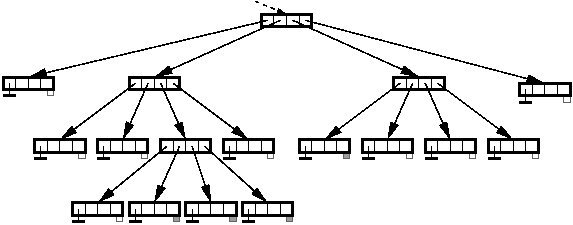
\includegraphics[scale=0.5]{quad_ref}
\caption{Zeigergeflecht eines Quadtree}
\label{abb_quad_ref}
\diaend

\subsubsection{Positionscodierung}
\label{pos_code}
Bei der Positionscodierung erh"alt jeder Knoten einen eindeutigen Index. 
F"ur die Sohnknoten muss eine bestimmte Reihenfolge definiert werden, woraus 
sich ein entsprechendes Nummerierungsschema ableitet.
H"aufig wird die Reihenfolge an Hand der Lebesgue-Kurve festgelegt. 
Der Index eines Knotens ist dann der Vektor, der sich aus Nummern der Knoten 
ergibt, die auf dem Pfad von der Wurzel zu ihm besucht wurden. 
Besonders anschaulich ist die Verwendung von Oktalzahlen f"ur den Index. 
Jede Ziffer gibt die Nummer des entsprechenden Sohnknotens wieder. Die Anzahl 
der Ziffern liefert die Tiefe des indizierten Knotens. Hiermit kann auch 
die Position der Zelle des Oktalbaums bestimmt werden, die dem Knoten 
zugeordnet ist. Hierher r"uhrt auch der Name Positionscodierung f"ur diese 
Repr"asentationsform. Abbildung \ref{abb_pos_quad}a) zeigt die 
Positionscodierung nach diesem Verfahren im 2-Dimensionalen zu einem Quadtree. 

Gegen"uber dem Zeigergeflecht ist die Identifikation von Knoten einfacher, 
woraus eine Vereinfachung verschiedener Algorithmen resultiert. 

In dieser Arbeit wird eine leicht abgewandelte Form benutzt, die besonders 
intuitiv ist und auf der das Normzellenschema leicht simuliert werden kann.
Es wird jede Raumrichtung gesondert betrachtet, wodurch ein 3-dimensionaler 
Vektor aus Bin"arzahlen entsteht. Somit wird f"ur jede Raumrichtung bestimmt, 
ob der Sohn im jeweils vorderen oder hinteren Teilraum liegt. 
Zus"atzlich wird noch die Knotenh"ohe im Index vermerkt (vgl. Abbildung 
\ref{abb_pos_quad}b). 

\diabeg[!t]
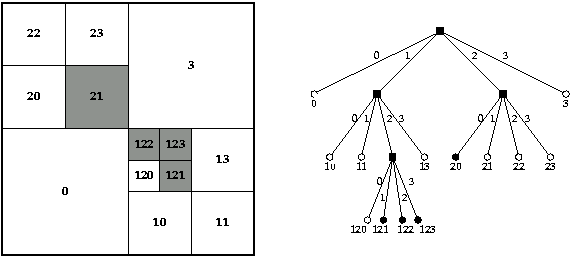
\includegraphics[scale=.75]{pos_quad_classic}
\begin{center}
\emph{a) "ublich}
\end{center}
\vspace{1.5em}
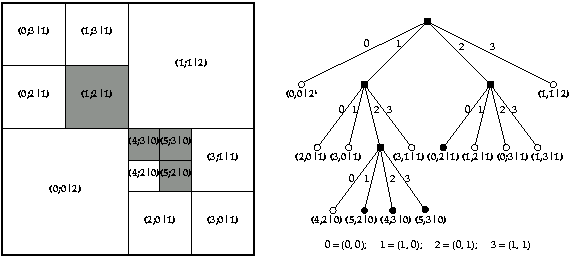
\includegraphics[scale=.75]{pos_quad_alt}
\begin{center}
\emph{b) in dieser Arbeit verwendet}
\end{center}
\caption{Positionscodierung}
\label{abb_pos_quad}
\diaend

Die Positionscodierung wird in der Literatur auch als \emph{linearer Code} 
oder \emph{leafcode} bezeichnet. 


\subsubsection{Codierung "uber Raum-Position und Gr"o"se}
Statt "uber den Pfad durch den Baum l"asst sich ein Knoten auch "uber seine 
Position $P$ im Raum und seine Gr"o"se $G$ identifizieren. Die Position 
kann dabei "uber die Koordinaten eines bestimmten Zellpunkts, "uber die Anzahl 
der Maschenweiten eines virtuellen Gitters feinster Aufl"osung oder durch 
eine Bin"aradresse "ahnlich der Positionscodierung dargestellt werden. 
Die Gr"o"se wird entweder durch die reale Gr"o"se oder ein Vielfaches der 
Maschenweite angegeben. 
Nachteilig an dieser Repr"asentationsform ist die fehlende Unterst"utzung des 
Organisationsprinzips Hierachie.

Der in Abbildung \ref{abb_pos_quad} dargestellte Quadtree k"onnte durch 
folgenden Code~$C=(P;G)$ dargestellt werden: 

\begin{tabularx}{\linewidth}{lX}
Bl"atter: & (0,~0;~4), (0,~4;~2), (0,~6;~2), (2,~4;~2), (2,~6;~2), (4,~0;~2), 
	    (4,~2; 1), (4,~3;~1), (4,~4;~4), (5,~2;~1), (5,~3;~1), (6,~0;~2), 
	    (6,~2;~2)\\
inner Knoten: & (0,~0;~8), (0,~4;~4), (4,~0;~4), (4,~2;~2)
\end{tabularx}

\subsubsection{Pr"aorder-Traversierung}
\label{pot_code}
Es gibt unterschiedliche Formen, um alle Knoten eines Baums abzulaufen, also 
zu traversieren. Durch Tiefensuche "uber den Baum entsteht, je nachdem ob 
dabei der Vaterknoten vor, in der Mitte oder nach den S"ohnen notiert wird, 
\emph{Pr"aorder-}, \emph{Inorder-} oder \emph{Postorder-Traversierung}. 
Wird Breitensuche angewendet, also alle Knoten einer Tiefe besucht, 
bevor ihre S"ohne besucht werden, entsteht eine 
\emph{Levelorder-Traversierung}.

F"ur Oktalb"aume wird dabei h"aufig die Pr"aorder-Traversierung verwendet. 
Da innere Knoten stets acht S"ohne besitzen, ist eine besonders kompakte 
Darstellung m"oglich: Beispielsweise k"onnen innere Knoten mit {\tt 1}, 
Bl"atter 
mit {\tt 0} markiert werden. 
Das zus"atzliche Farbattribut wird einfach hinter die blattmarkierende {\tt 0} 
hinzugef"ugt. Damit liegt der Oktalbaum sehr kompakt in einer linearisierten 
Form vor und kann somit als bin"arer Strom (binary Stream) verarbeitet werden. 

Mit dieser Codierung ergibt sich f"ur den Quadtree aus Abbildung 
\ref{abb_pos_quad}:
\begin{alltt}
1001000 01000101 01001010 0000000
\end{alltt}

Die Pr"aorder-Traversierung wird auch Depth-First-Strategie genannt. In der 
Literatur kommen auch die Namen \emph{DF-expression} oder \emph{treecode} f"ur 
diese Form der Codierung vor.

\subsection{Operationen auf Oktalb"aumen}
Neben den im Abschnitt \ref{basis_op_beg} beschriebenen grundlegenden 
Operationen, gibt es weitere Grundoperationen auf einem Oktalbaum.
Hierzu geh"oren das Erzeugen, L"oschen oder die Aufspaltung eines Blatts, 
sowie die Vereinigung gleichgef"arbter Bl"atter zu einem Blatt der 
dar"uberliegenden Ebene (Kompaktieren). Diese Operationen sind auf den hier 
verwendeten Zeigergeflecht als Basisstruktur leicht effizient zu realisieren. 

Raumpartitionierende Strukturen -- und somit der Oktalbaum -- sind geradezu 
pr"adestiniert f"ur die bin"aren Mengenoperationen Schnitt, Vereinigung 
und Differenz: Die beiden B"aume werden synchron (z.B. durch 
Pr"aorder-Traversierung) durchlaufen und an den Bl"attern entsprechende 
Vergleiche durchgef"uhrt, um so den resultierenden Baum zu konstruieren. 
In der Literatur finden sich auch effiziente Algorithmen zur Realisierung der 
affinen Transformationen Translation, Rotation und Skalierung. 

Des Weiteren ist die Bestimmung der Nachbarzelle zu einem Oktalbaumknoten 
von Bedeutung. 
Die Nachbarzelle ist jedoch nicht direkt aus der Oktalbaumstruktur ersichtlich, 
insbesondere wenn diese durch ein Zeigergeflecht repr"asentiert wird. Hierf"ur 
wird die Positionscodierung verwendet. Mit dem in dieser Arbeit verwendeten 
Index (vgl. Abschnitt \emph{Positionscodierung} \vpageref{pos_code}) kann 
leicht der entsprechende 'theoretische' Nachbar auf gleicher Ebene ermittelt 
werden. Der so ermittelte Nachbar kann jedoch unterhalb des 'realen' Nachbars 
liegen, wenn der entsprechende Baumast nicht so tief ist wie der 
Ausgangsknoten. 
Mit Hilfe von \funcdef{getExistNode}{NodeIndex p}{NodeIndex} 
(\algref{alg_getexistnode_idx}) wird deshalb der Index des tiefsten 
existierenden Knotens ermittelt, der sich auf dem Pfad zu \param{p} befindet. 
Der so gefundene Knoten muss jedoch nicht ein Blatt sein. Diese k"onnen durch 
rekursiven Abstieg zu den entsprechenden S"ohnen (Gegenrichtung als die 
Richtung zum Nachbarn) gefunden werden.

Es finden sich Algorithmen, die einen balancierten Oktalbaum voraussetzen. 
\emph{Balanciert} bedeutet, dass sich die Maschenweite zweier benachbarten 
Zellen um maximal den Faktor $2$ unterscheiden (also die Tiefe von 
Nachbarknoten maximal um $\pm 1$ differiert). 
Da sich Aufspaltungen oder Vereinigungen 
innerhalb einer Zelle bei der Balancierung h"ochstens auf deren 
Nachbarzellen auswirken, haben "Anderungen im Baum nur lokale Wirkung. 
Somit l"asst sich die Balancierung eines Baums effizient umsetzen.

Zur Aufz"ahlung r"aumlich angeordneter diskreter Daten -- entsprechend 
der Lebesgue-Kurve -- kann der \emph{Morton-Index} verwendet werden. 
Als herausragende Eigenschaft ist zu nennen, dass Nachbarschaftsbeziehungen 
in einer so erzeugenden Sequenz bereits im urspr"unglichen Baum vorhanden
waren. 
Der Morton-Index kann so effizient zur Nachbarschaftsbestimmung von Knoten 
im Oktalbaum genutzt werden und eignet sich zur dimensionsunabh"angigen 
Sequentialisierung von Quad-/Octree-Zeigerstrukturen. 
Ferner kann der Morton-Index zur 
Oktalbaumgenerierung aus einem 
Normzellen-Aufz"ahlungsschema verwendet werden.

%% End of Document


%% End of Document
